\documentclass[12pt,a4paper,oneside]{report}
\usepackage[utf8]{inputenc}
\usepackage[T1]{fontenc}
\usepackage{lmodern}
\usepackage[a4paper,left=3.5cm,right=2.5cm,top=3cm,bottom=3cm]{geometry}
\usepackage{graphicx}
\usepackage{booktabs}
\usepackage{longtable}
\usepackage{array}
\usepackage{tabularx}
\usepackage{float}
\usepackage{xcolor}
\usepackage{hyperref}
\usepackage{listings}
\usepackage{setspace}
\usepackage{enumitem}

% Update these fields before formal submission.
\newcommand{\thesistype}{Bachelor Thesis}
\newcommand{\thesistitle}{Design and Implementation of Anhoc}
\newcommand{\thesissubtitle}{A Web-Based Mathematics Learning Platform for Structured Learning, Adaptive Practice, and Progress Tracking}
\newcommand{\thesisstudent}{Your Name}
\newcommand{\thesisstudentid}{Your Student ID}
\newcommand{\thesisspecialty}{Information and Communication Technology}
\newcommand{\thesissupervisor}{Your Supervisor}
\newcommand{\thesislocation}{Ho Chi Minh City}
\newcommand{\thesismonthyear}{June 2026}

\hypersetup{
  colorlinks=true,
  linkcolor=blue,
  urlcolor=blue,
  pdftitle={Design and Implementation of Anhoc},
  pdfauthor={Your Name}
}

\graphicspath{{docs/thesis/chapters/}{docs/thesis/}{docs/images/}{docs/}}
\setstretch{1.2}
\setlength{\parindent}{1.5em}
\setlength{\parskip}{0.35em}
\setlist[itemize]{topsep=0.35em,itemsep=0.15em}
\setlist[enumerate]{topsep=0.35em,itemsep=0.15em}

\newcommand{\code}[1]{\nolinkurl{#1}}
\newcolumntype{L}[1]{>{\raggedright\arraybackslash}p{#1}}
\newcolumntype{Y}{>{\raggedright\arraybackslash}X}

\lstdefinestyle{thesiscode}{
  basicstyle=\ttfamily\small,
  breaklines=true,
  columns=fullflexible,
  keepspaces=true,
  frame=single,
  rulecolor=\color{black!20}
}

\begin{document}

\hypersetup{pageanchor=false}
\begin{titlepage}
\thispagestyle{empty}
\begin{center}
{\Large UNIVERSITY OF SCIENCE AND TECHNOLOGY OF HANOI\par}
\vspace{0.35cm}
{\large BACHELOR'S DEGREE\par}

\vspace{2.1cm}
{\LARGE \textbf{\thesistype}\par}

\vspace{1.25cm}
{\large by\par}
\vspace{0.4cm}
{\Large \textbf{\thesisstudent}\par}
{\large \thesisstudentid\par}
\vspace{0.3cm}
{\large \thesisspecialty\par}

\vspace{1.6cm}
{\large Title:\par}
\vspace{0.35cm}
{\Large \textbf{\thesistitle}\par}
\vspace{0.5cm}
{\large \thesissubtitle\par}

\vspace{1.8cm}
\begin{tabular}{rl}
Supervisor: & \thesissupervisor \\
Project basis: & Anhoc web application repository \\
Implementation scope: & \code{frontend/}, \code{backend/}, and \code{chatbot/}
\end{tabular}

\vfill
{\thesislocation. \thesismonthyear\par}
\end{center}
\end{titlepage}

\chapter*{Declaration}
\thispagestyle{empty}
I hereby declare that this thesis titled \textit{\thesistitle} is prepared from the implemented
Anhoc repository and the accompanying project documentation. All architectural descriptions,
feature summaries, and implementation details presented in this report are derived from the
inspected codebase, and external concepts or technologies are cited where appropriate.

To the best of my knowledge, this report does not intentionally reproduce uncited work as an
original contribution. Any frameworks, libraries, documents, or external references used in the
preparation of this thesis are acknowledged in the bibliography.

\vfill
\begin{flushright}
\thesislocation, \thesismonthyear\\[2cm]
\textbf{\thesisstudent}
\end{flushright}

\chapter*{Acknowledgements}
\thispagestyle{empty}
This thesis was prepared from the current Anhoc web application repository. The document reflects
the work embodied in the frontend, backend, database, and chatbot modules, as well as the
supporting technical design notes maintained with the project.

I would like to acknowledge the contributors who shaped the platform's architecture, educational
workflows, and deployment configuration, together with the maintainers of the open-source tools
that made the system possible, including Next.js, React, Express, Prisma, PostgreSQL, and the
supporting Python ecosystem used by the tutoring service.

\vfill
\begin{flushright}
(\thesisstudent)\\
\thesislocation, \thesismonthyear
\end{flushright}
\clearpage
\tableofcontents
\thispagestyle{empty}

\clearpage
\pagenumbering{roman}
\setcounter{page}{1}

\chapter*{List of Acronyms}
\addcontentsline{toc}{chapter}{List of Acronyms}
\begin{longtable}{L{0.22\textwidth}L{0.68\textwidth}}
\textbf{API} & Application Programming Interface \\
\textbf{BYOK} & Bring Your Own Key \\
\textbf{CORS} & Cross-Origin Resource Sharing \\
\textbf{JWT} & JSON Web Token \\
\textbf{LLM} & Large Language Model \\
\textbf{ORM} & Object-Relational Mapping \\
\textbf{RBAC} & Role-Based Access Control \\
\textbf{REST} & Representational State Transfer \\
\textbf{UI} & User Interface \\
\textbf{XP} & Experience Points \\
\end{longtable}

\clearpage
\addcontentsline{toc}{chapter}{List of Figures}
\listoffigures

\clearpage
\addcontentsline{toc}{chapter}{List of Tables}
\listoftables

\clearpage
\chapter*{Abstract}
\addcontentsline{toc}{chapter}{Abstract}
Anhoc is a web-based mathematics learning platform designed for structured school-level study. The
implemented system combines bilingual lesson content, dynamically generated practice exercises,
grade-level tests, progression tracking, administrative management, notifications, multiplayer and
single-player math games, and an integrated tutoring chatbot. This thesis documents the design
and implementation of Anhoc based on the current repository contents.

The software follows a service-oriented web architecture. A Next.js frontend provides the student
and administrative interfaces. An Express backend exposes REST endpoints for authentication,
lessons, tests, achievements, notifications, games, supervisor workflows, and subscription
management. Prisma is used as the persistence layer, PostgreSQL stores the core application
state, and a companion Python chatbot service extends the platform with conversational tutoring
capabilities.

A notable implementation decision is the use of persisted question snapshots. Reusable templates
define how questions are generated, while snapshots preserve the exact generated variables,
accepted answers, and scoring outcomes for each attempt. This design supports reproducible
grading, debugging, review, and reporting. The project also adopts dynamic role-based access
control with subject-level restrictions, progression services for mastery and XP, and operational
support for learn units and subscription-oriented platform management.

This thesis presents the problem context, requirements, system architecture, data model,
implementation details, and an evaluation of the current solution. It also discusses limitations
and practical improvements required to mature the platform further as an educational software
system.

\textbf{Keywords:} mathematics learning platform, question generation, role-based access control,
progress tracking, tutoring chatbot, web application architecture

\clearpage
\hypersetup{pageanchor=true}
\pagenumbering{arabic}

\chapter{Introduction}

\section{Background}

Digital learning systems are increasingly expected to do more than present static content. In mathematics education, students need repeated practice, immediate feedback, structured progression, and content that can be adapted to multiple grades and topics. A conventional content website can display lessons, but it does not by itself provide reusable question generation, mastery tracking, or administrative control over subject-specific learning material.

The Anhoc project addresses this gap by combining theory lessons, generated practice, formal test sessions, and gamified progression in a single web application. The project targets school-level mathematics learning and is organized around subjects, grades, and lessons. The implemented system allows a student to read theory content, start practice from lesson templates, submit answers, complete tests, and monitor progress through XP, levels, and achievements. At the same time, an administrator can manage lessons, question templates, user accounts, roles, and access permissions.

\subsection{Statistical Context of E-Learning in Vietnam}

The Vietnamese context makes digital learning both promising and uneven. DataReportal reported 78.44 million internet users in Vietnam in January 2024, equivalent to 79.1\% of the population, together with 168.5 million active cellular mobile connections \cite{datareportal-vietnam-2024}. This creates a strong baseline for mobile-first learning applications. UNESCO also reported that about nine out of ten schools in Vietnam are connected to the internet and that national policy targets full school connectivity by 2025 \cite{unesco-vietnam-technology}. EdTech Hub's 2024 rapid scan further notes that the Vietnamese educational technology landscape already includes online learning platforms, learning apps, websites, and video-based resources, showing that e-learning is no longer a niche delivery mode in the country \cite{edtechhub-vietnam-scan}.

However, the same sources show that access and quality remain unequal. UNESCO highlights a very large home-access gap: 95\% of children from the richest households benefit from internet access at home compared with only 18\% of children from the poorest households. During the COVID-19 period, students from the poorest households were also 34\% less likely to experience distance learning than students from the richest households, and there were roughly three students per computer on average \cite{unesco-vietnam-technology}. A World Bank case note on Vietnam's emergency distance-learning response adds that, in less advantaged areas, only 10\% to 20\% of students and teachers had access to personal digital devices at home, even though some provinces still managed to reach about 80\% of students through a combination of online and educational television lessons \cite{worldbank-vietnam-distance-learning,worldbank-vietnam-tv-learning}.

\section{Problem Statement}

The main engineering problem solved by Anhoc is the design of a learning platform that satisfies four requirements at the same time:
\begin{itemize}
  \item it must support reusable content across grades and subjects;
  \item it must generate exercises dynamically rather than storing every question instance manually;
  \item it must keep each attempt stable enough to be scored, reviewed, and audited later;
  \item it must provide operational control for administrators without hard-coding every permission into the user interface.
\end{itemize}

Many simple practice applications solve only one part of this problem. They either store fixed question banks, do not track long-term student progression, or rely on coarse user roles that become difficult to extend. Anhoc introduces a more structured approach by combining generated questions with persisted snapshots, dynamic role-based access control, and a progression subsystem.

\subsection{Advantages and Limitations of E-Learning Applications in Vietnam}

The statistical context above suggests several clear advantages for e-learning applications in Vietnam.
\begin{itemize}
  \item \textbf{Large reachable user base:} high internet penetration and widespread mobile connectivity make app-based learning distribution technically feasible at national scale \cite{datareportal-vietnam-2024}.
  \item \textbf{Institutional readiness:} the fact that most schools are already connected to the internet creates a practical foundation for blended learning, school-supported digital homework, and platform-assisted assessment \cite{unesco-vietnam-technology}.
  \item \textbf{Flexible continuity:} emergency distance-learning evidence shows that digital tools, especially when combined with broadcast channels, can preserve instructional continuity during disruption \cite{worldbank-vietnam-tv-learning}.
  \item \textbf{Expanding ecosystem:} the presence of platforms, apps, websites, and video channels indicates that learners and schools are already familiar with multiple forms of educational technology \cite{edtechhub-vietnam-scan}.
\end{itemize}

At the same time, e-learning applications in Vietnam face structural limitations that directly motivate Anhoc's design.
\begin{itemize}
  \item \textbf{Access inequality:} home internet access and device ownership vary sharply by income and geography, which means an app cannot assume stable, private, always-on access for every learner \cite{unesco-vietnam-technology,worldbank-vietnam-distance-learning}.
  \item \textbf{Fragmentation of tools and content:} World Bank analysis of Vietnamese e-learning practice notes underdeveloped, unstandardized platforms and inconsistent learning materials, making quality assurance difficult \cite{worldbank-vietnam-distance-learning}.
  \item \textbf{Weak progression support in basic tools:} many digital offerings can deliver lessons or quizzes but do not reliably connect content, assessment history, progression, and administration in one coherent system.
  \item \textbf{Equity risk:} if platform design ignores device constraints, bandwidth limits, or administrative coordination, digital learning can widen rather than reduce educational inequality \cite{unesco-vietnam-technology,worldbank-vietnam-distance-learning}.
\end{itemize}

These conditions shape the problem statement for Anhoc. A useful platform in Vietnam must not only digitize lessons; it must also provide structured practice, durable assessment records, scalable administration, and a design that remains usable in a context where digital opportunity and digital inequality coexist.

\section{Objectives}

This thesis has the following objectives:
\begin{itemize}
  \item document the implemented Anhoc system in a thesis-style format;
  \item explain the architecture and data model used by the project;
  \item describe how the platform generates and evaluates mathematical exercises;
  \item analyze how authentication, authorization, and administration are handled;
  \item evaluate the strengths, limitations, and next steps of the current implementation.
\end{itemize}

\section{Scope}

The scope of this thesis is limited to the code and documentation available in the repository. It focuses on the currently implemented frontend, backend, database schema, and operational flows. The thesis does not claim to measure learning outcomes through classroom experimentation, because no such experimental dataset is included in the repository. Evaluation is therefore based on software capabilities, system structure, and scenario-level validation.

\section{Contributions of the Project}

The implemented project contributes several concrete software ideas:
\begin{itemize}
  \item a bilingual lesson structure for educational content in English and Vietnamese;
  \item a question-template model that supports variables, derived expressions, constraints, and multiple accepted formulas;
  \item persisted question snapshots that separate reusable templates from concrete attempt data;
  \item a progression model combining mastery, XP logs, levels, and achievements;
  \item a dynamic access-control model that separates actions, resources, and subject restrictions.
\end{itemize}

\section{Thesis Structure}

The remainder of this thesis is organized as follows. Chapter 2 presents the requirements and analysis of the project domain. Chapter 3 describes the system design, architecture, security model, and data model. Chapter 4 explains implementation details across the frontend, backend, and database layers. Chapter 5 evaluates the current solution through representative scenarios, strengths, and limitations. Chapter 6 concludes the thesis and outlines future work.

\section{Requirements Analysis}

\subsection{Stakeholders and User Roles}

The primary stakeholders in Anhoc are students, administrators, and maintainers of the platform.

\begin{itemize}
  \item Students consume learning content, complete exercises, take tests, and monitor progress.
  \item Administrators maintain educational content, templates, users, roles, and reports.
  \item Maintainers operate the deployment, database, and system configuration.
\end{itemize}

The codebase also distinguishes between global roles and subject-specific permissions. This is important because a role may have permission to manage some resources without necessarily having access to all subjects.

\subsection{Functional Requirements}

Table \ref{tab:functional-requirements} summarizes the main functional requirements derived from the implementation.

\begin{table}[H]
\centering
\caption{Core functional requirements}
\label{tab:functional-requirements}
\begin{tabularx}{\textwidth}{L{0.18\textwidth}Y}
\toprule
\textbf{Area} & \textbf{Requirement} \\
\midrule
Authentication & The system shall allow user registration, login, profile retrieval, password change, and activity retrieval. \\
Lessons & The system shall support subject and grade organization, lesson listing, lesson detail retrieval, and lesson authoring by authorized users. \\
Practice & The system shall generate lesson-based practice attempts from reusable templates and store concrete snapshot records for each generated question. \\
Testing & The system shall create grade-level test attempts, support answer submission, and compute final scores on completion. \\
Templates & The system shall support creation, update, deletion, preview, reporting, and review of question templates. \\
Progression & The system shall track study time, mastery status, XP, levels, and achievements. \\
Administration & The system shall provide user, role, permission, subject-access, and dashboard management endpoints. \\
\bottomrule
\end{tabularx}
\end{table}

\subsection{Use Case Model}

Figure \ref{fig:use-case-diagram} summarizes the main interactions between the implemented role groups and the platform boundary. The repository defines five fixed application roles: \code{free\_student}, \code{sub\_student}, \code{teacher}, \code{supervisor}, and \code{admin}. A guest actor is also useful in the requirements model because registration and login begin before an authenticated role is established.

\begin{figure}[H]
\centering
\resizebox{0.82\textwidth}{!}{
\begin{tikzpicture}[node distance=1.0cm and 1.1cm]
  \node[usecase, minimum width=4.6cm] (uc1) at (6.8,13.8) {Register or\\Login};
  \node[usecase, minimum width=4.6cm] (uc2) at (6.8,11.7) {Study\\Lesson};
  \node[usecase, minimum width=4.6cm] (uc3) at (6.8,9.6) {Complete\\Lesson Practice};
  \node[usecase, minimum width=4.6cm] (uc4) at (6.8,7.5) {Take Grade-Level\\Test};
  \node[usecase, minimum width=4.6cm] (uc5) at (6.8,5.4) {View Progress and\\Achievements};
  \node[usecase, minimum width=4.6cm] (uc6) at (6.8,3.3) {Manage Content and\\Question Templates};
  \node[usecase, minimum width=4.6cm] (uc7) at (6.8,1.4) {Manage Learning Unit\\Members and Seats};
  \node[usecase, minimum width=4.6cm] (uc8) at (6.8,-0.9) {Manage Roles, Access\\Control, and Dashboard};

  \node[systembox, fit=(uc1) (uc2) (uc3) (uc4) (uc5) (uc6) (uc7) (uc8), inner xsep=1.4cm, inner ysep=1.2cm] (system) {};
  \node[anchor=north west] at ($(system.north west)+(0.2,-0.2)$) {\textbf{Anhoc Platform}};

  \node[actor] (guest) at (0,13.2) {Guest};
  \node[actor] (free) at (0,10.9) {Free\\Student};
  \node[actor] (sub) at (0,8.6) {Subscribed\\Student};
  \node[actor] (teacher) at (13.6,10.9) {Teacher};
  \node[actor] (supervisor) at (13.6,8.6) {Supervisor};
  \node[actor] (admin) at (13.6,6.3) {Administrator};

  \draw (guest.east) -- (uc1.west);
  \draw (free.east) -- (uc1.west);
  \draw (free.east) -- (uc2.west);
  \draw (free.east) -- (uc3.west);
  \draw (free.east) -- (uc4.west);
  \draw (free.east) -- (uc5.west);
  \draw (sub.east) -- (uc2.west);
  \draw (sub.east) -- (uc3.west);
  \draw (sub.east) -- (uc4.west);
  \draw (sub.east) -- (uc5.west);

  \draw (teacher.west) -- (uc1.east);
  \draw (teacher.west) -- (uc6.east);
  \draw (supervisor.west) -- (uc1.east);
  \draw (supervisor.west) -- (uc6.east);
  \draw (supervisor.west) -- (uc7.east);
  \draw (admin.west) -- (uc1.east);
  \draw (admin.west) -- (uc6.east);
  \draw (admin.west) -- (uc7.east);
  \draw (admin.west) -- (uc8.east);
\end{tikzpicture}
}
\caption{Use case diagram of the Anhoc platform}
\label{fig:use-case-diagram}
\end{figure}

\subsection{Use Case Descriptions}

\subsubsection{Use Case 1: Register or Login}

\begin{longtable}{L{0.28\textwidth}L{0.62\textwidth}}
\textbf{Primary actor} & Guest or authenticated platform user \\ \hline
\textbf{Goal} & Create an account or obtain a valid authenticated session. \\ \hline
\textbf{Preconditions} & The user has network access to the frontend and backend services. Login additionally requires an existing account. \\ \hline
\textbf{Trigger} & The user opens the authentication area and submits a registration or login form. \\ \hline
\textbf{Main flow} & (1) The user chooses registration or login. (2) The frontend sends credentials and requested role information to the authentication API. (3) The backend validates the request, resolves the target role, and loads permission data. (4) The backend returns session tokens and profile information. (5) The frontend stores the session and redirects the user to the proper interface. \\ \hline
\textbf{Postconditions} & A new account is created or an authenticated session is established with role-specific permissions. \\
\end{longtable}

\subsubsection{Use Case 2: Study Lesson}

\begin{longtable}{L{0.28\textwidth}L{0.62\textwidth}}
\textbf{Primary actor} & Free student or subscribed student \\ \hline
\textbf{Goal} & Read lesson content for a chosen subject, grade, and lesson. \\ \hline
\textbf{Preconditions} & The student is authenticated and has access to the selected subject. \\ \hline
\textbf{Trigger} & The student opens a lesson from the learning area. \\ \hline
\textbf{Main flow} & (1) The student browses grades and lessons. (2) The frontend requests lesson detail from the API. (3) The backend retrieves lesson metadata and markdown content. (4) The frontend renders the bilingual lesson page. (5) The frontend records study time while the student remains on the page. \\ \hline
\textbf{Postconditions} & The lesson is displayed and study progress can be updated for the student. \\
\end{longtable}

\subsubsection{Use Case 3: Complete Lesson Practice}

\begin{longtable}{L{0.28\textwidth}L{0.62\textwidth}}
\textbf{Primary actor} & Free student or subscribed student \\ \hline
\textbf{Goal} & Practice a lesson through generated questions and receive feedback. \\ \hline
\textbf{Preconditions} & The student is authenticated and the lesson has available question templates. \\ \hline
\textbf{Trigger} & The student starts practice from a lesson page. \\ \hline
\textbf{Main flow} & (1) The frontend requests a practice attempt for the lesson. (2) The backend generates question snapshots from the lesson templates. (3) The student answers questions one by one. (4) The frontend submits responses. (5) The backend evaluates correctness, computes the score, updates mastery and XP, and checks achievements. (6) The result view is returned to the student. \\ \hline
\textbf{Postconditions} & The attempt is stored with snapshot-level grading and the student progression state is updated. \\
\end{longtable}

\subsubsection{Use Case 4: Take Grade-Level Test}

\begin{longtable}{L{0.28\textwidth}L{0.62\textwidth}}
\textbf{Primary actor} & Free student or subscribed student \\ \hline
\textbf{Goal} & Assess broader understanding across the lessons of one grade. \\ \hline
\textbf{Preconditions} & The student is authenticated and the grade has enough templates to assemble a test. \\ \hline
\textbf{Trigger} & The student chooses a grade test from the practice or testing area. \\ \hline
\textbf{Main flow} & (1) The frontend requests a grade-level test attempt. (2) The backend collects eligible templates from lessons in the grade. (3) Question snapshots are generated for the attempt. (4) The student submits answers. (5) The backend finalizes the attempt, calculates the score, and records progression outcomes. \\ \hline
\textbf{Postconditions} & A completed grade-level test attempt is stored and can be reviewed later. \\
\end{longtable}

\subsubsection{Use Case 5: View Progress and Achievements}

\begin{longtable}{L{0.28\textwidth}L{0.62\textwidth}}
\textbf{Primary actor} & Free student or subscribed student \\ \hline
\textbf{Goal} & Review learning progress, XP history, mastery, and earned achievements. \\ \hline
\textbf{Preconditions} & The student is authenticated and has recorded activity in the system. \\ \hline
\textbf{Trigger} & The student opens the dashboard, profile, or achievements page. \\ \hline
\textbf{Main flow} & (1) The frontend requests student statistics and achievement data. (2) The backend loads profile, activity, mastery, and achievement records. (3) The frontend renders summary cards and achievement states. \\ \hline
\textbf{Postconditions} & The student can inspect current progress and earned rewards. \\
\end{longtable}

\subsubsection{Use Case 6: Manage Content and Question Templates}

\begin{longtable}{L{0.28\textwidth}L{0.62\textwidth}}
\textbf{Primary actor} & Teacher, supervisor, or administrator \\ \hline
\textbf{Goal} & Maintain lessons and reusable question templates for the learning platform. \\ \hline
\textbf{Preconditions} & The actor is authenticated and has the required lesson or test management permissions within the permitted subject scope. \\ \hline
\textbf{Trigger} & The actor creates, updates, previews, or deletes a lesson or template in a management interface. \\ \hline
\textbf{Main flow} & (1) The actor edits lesson or template data in the frontend. (2) The frontend sends the request to the backend. (3) The backend validates the JWT, permissions, and subject scope. (4) The backend persists the changes in the database. (5) The frontend refreshes the management view. \\ \hline
\textbf{Postconditions} & The affected content records are updated and become available to the rest of the platform. \\
\end{longtable}

\subsubsection{Use Case 7: Manage Learning Unit Members and Seats}

\begin{longtable}{L{0.28\textwidth}L{0.62\textwidth}}
\textbf{Primary actor} & Supervisor or administrator \\ \hline
\textbf{Goal} & Manage a learning unit by purchasing seats and creating member accounts. \\ \hline
\textbf{Preconditions} & The actor is authenticated, has supervisor-level access, and is associated with a learn unit or is acting as an administrator over one. \\ \hline
\textbf{Trigger} & The actor opens the member management area or seat management flow. \\ \hline
\textbf{Main flow} & (1) The actor requests the current learn unit context. (2) The frontend sends member or seat management operations to the supervisor API. (3) The backend checks whether the user is the relevant supervisor or an administrator. (4) The backend updates seat counts, subscription records, or member accounts. (5) The frontend refreshes the roster and learn unit summary. \\ \hline
\textbf{Postconditions} & Learning unit seats or member accounts are updated consistently with subscription and scope constraints. \\
\end{longtable}

\subsubsection{Use Case 8: Manage Roles, Access Control, and Dashboard}

\begin{longtable}{L{0.28\textwidth}L{0.62\textwidth}}
\textbf{Primary actor} & Administrator \\ \hline
\textbf{Goal} & Control platform-wide users, roles, permissions, subject access, and aggregate reports. \\ \hline
\textbf{Preconditions} & The administrator is authenticated with full management privileges. \\ \hline
\textbf{Trigger} & The administrator opens the admin dashboard or a user and permission management screen. \\ \hline
\textbf{Main flow} & (1) The administrator requests role, user, or dashboard data. (2) The frontend calls the admin API. (3) The backend validates administrative authority. (4) The backend loads or updates users, roles, permissions, and statistical summaries. (5) The frontend renders the resulting dashboard or management state. \\ \hline
\textbf{Postconditions} & Platform-level administration data is viewed or updated with persistent RBAC changes. \\
\end{longtable}

\subsection{Non-Functional Requirements}

The repository implies the following non-functional requirements:

\begin{itemize}
  \item \textbf{Modularity:} frontend, backend, persistence, and progression logic should remain separable.
  \item \textbf{Consistency:} generated questions must remain stable after creation so that grading and reporting are reproducible.
  \item \textbf{Security:} protected endpoints require JWT-based authentication and permission checks.
  \item \textbf{Extensibility:} roles, actions, resources, and subject restrictions should be data-driven rather than hard-coded.
  \item \textbf{Deployability:} the architecture should run in a common cloud arrangement using Vercel, Render, and Neon.
\end{itemize}

\subsection{Learning Content Requirements}

Educational content in Anhoc is organized around a hierarchy of subjects, grades, and lessons. Lessons contain bilingual titles and markdown-based content bodies. This leads to several domain requirements:

\begin{itemize}
  \item one lesson belongs to one grade and one subject;
  \item lesson content should be readable in more than one language;
  \item practice content should be attached to lessons through question templates rather than embedded into the lesson body itself;
  \item progress should be measurable at the lesson level.
\end{itemize}

\subsection{Assessment Requirements}

Assessment in the project has two modes:
\begin{itemize}
  \item lesson-based practice for targeted repetition;
  \item grade-level tests for broader assessment across available lesson templates.
\end{itemize}

The assessment subsystem must support question generation, answer submission, correctness evaluation, score calculation, and post-completion progression updates. The implementation also needs to distinguish between theoretical questions and computed math questions because the grading strategy differs between those two cases.

\subsection{Administrative Requirements}

Administrative functionality in Anhoc goes beyond simple content editing. The platform must manage:
\begin{itemize}
  \item users and their assigned roles;
  \item permissions by action and resource;
  \item subject-level restrictions per role;
  \item dashboard statistics and user insights;
  \item reports submitted for problematic generated questions.
\end{itemize}

This requirement set justifies the presence of a dynamic RBAC model instead of a fixed boolean admin flag.

\subsection{Operational Assumptions}

The codebase assumes a web-first deployment model:
\begin{itemize}
  \item the frontend is delivered as a Next.js application;
  \item the backend exposes REST endpoints under \code{/api/v1};
  \item PostgreSQL is the source of truth for transactional and analytical learning data;
  \item environment variables define API URLs, CORS origins, JWT secret material, and achievement seeding behavior.
\end{itemize}

These assumptions shape the rest of the architecture described in the next chapter.

\chapter{System Design}

\section{Architectural Overview}

Anhoc uses a three-tier web architecture. A Next.js frontend provides the user interface. An Express backend exposes REST endpoints and business logic. PostgreSQL stores content, user identities, generated snapshots, and progression data. Prisma acts as the ORM boundary between the backend and the database.

\begin{figure}[H]
\centering
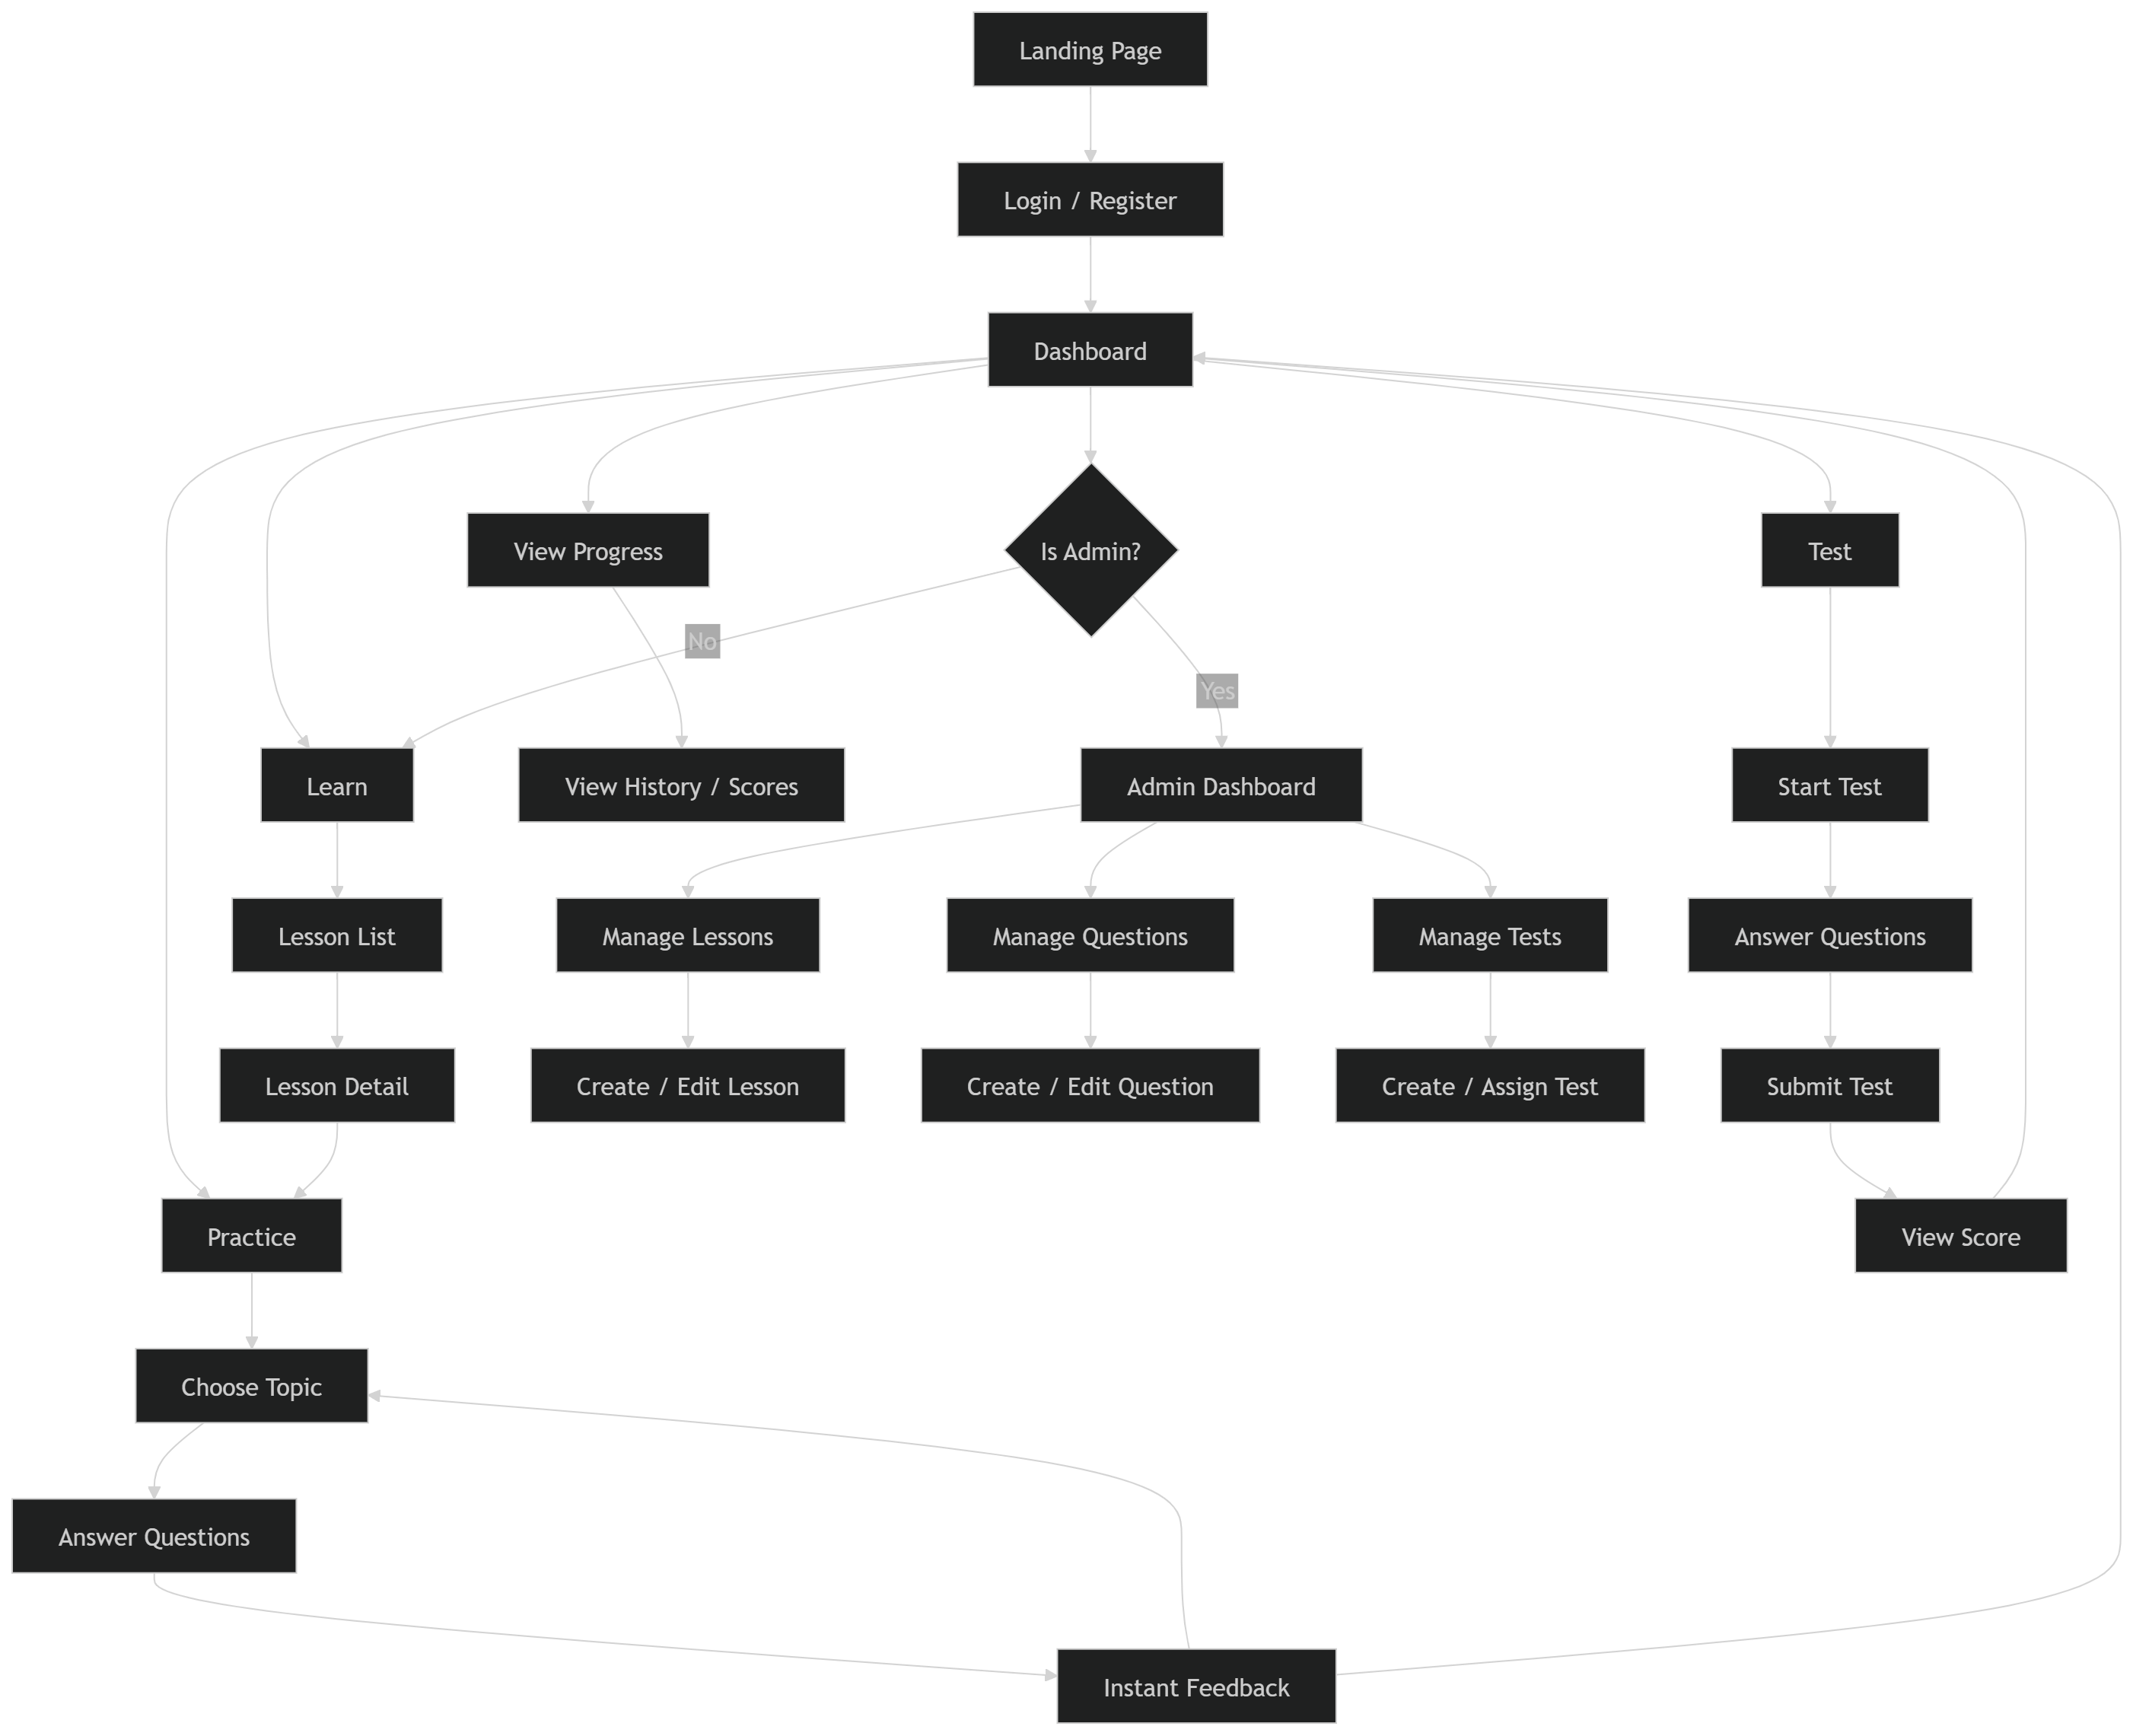
\includegraphics[width=0.9\textwidth]{../../images/anhoc-user-flow.png}
\caption{User-facing flow of the Anhoc platform}
\label{fig:user-flow}
\end{figure}

At a high level, the request flow is:
\begin{enumerate}
  \item the browser interacts with the Next.js frontend;
  \item the frontend calls backend routes under \code{/api/v1};
  \item the backend validates identity and permissions;
  \item business services coordinate data access and progression updates;
  \item PostgreSQL persists authoritative state.
\end{enumerate}

\section{Deployment Design}

The repository documents a practical deployment split:
\begin{itemize}
  \item Vercel hosts the frontend runtime;
  \item Render hosts the Node.js API;
  \item Neon provides PostgreSQL infrastructure.
\end{itemize}

This split is appropriate for a full-stack TypeScript project because it separates the static or server-rendered frontend from the API runtime and keeps the relational database independent of either application tier.

\section{Backend Design}

The backend entry point is \code{backend/server.ts}. It initializes Express, configures CORS, enables JSON parsing, mounts route modules, exposes a health endpoint, and conditionally seeds achievements at startup. The route structure is organized by domain:

\begin{itemize}
  \item \code{auth.ts} for identity, login, and profile operations;
  \item \code{lessons.ts} for educational content and practice initiation;
  \item \code{tests.ts} for attempts, answer submission, template management, and reports;
  \item \code{admin.ts} for users, roles, access control, and statistics;
  \item \code{achievements.ts} for achievement retrieval and re-evaluation.
\end{itemize}

This separation keeps HTTP concerns close to route boundaries while pushing calculation-heavy logic into services.

\section{Frontend Design}

The frontend is built with Next.js using an app-router structure under \code{frontend/src/app}. It includes separate areas for authentication, student flows, and administration. The frontend is supported by Axios-based service modules, Redux state for authentication and permissions, and feature-specific components such as lesson cards, question players, result modals, and achievement galleries.

From a design perspective, the frontend acts as an orchestration layer:
\begin{itemize}
  \item it collects user input and triggers backend operations;
  \item it renders lesson, practice, test, and admin views;
  \item it persists authentication tokens in browser storage and cookies;
  \item it enforces route-level and component-level access decisions using the permission payload returned by the backend.
\end{itemize}

\section{Security Model}

Authentication is handled with JWT bearer tokens. The middleware in \code{backend/middleware/auth.ts} extracts the token from the \code{Authorization} header, verifies it using the configured secret, and attaches the decoded payload to the request object.

Authorization is layered on top of authentication. The project uses:
\begin{itemize}
  \item role identity for coarse-grained decisions;
  \item grouped resource permissions for action checks;
  \item subject-level role restrictions for scoped access;
  \item helper middleware such as \code{isAdmin} and \code{selfOrAdmin}.
\end{itemize}

The design choice to keep permissions data-driven is significant. It allows new resources and actions to be introduced through database records and route logic instead of forcing the codebase into a rigid two-role system.

\section{Data Model}

The database schema in \code{backend/prisma/schema.prisma} defines the educational, assessment, and progression domain. Table \ref{tab:main-entities} summarizes the most important entities.

\begin{longtable}{L{0.28\textwidth}L{0.62\textwidth}}
\caption{Main persistent entities}\label{tab:main-entities}\\
\toprule
\textbf{Entity} & \textbf{Purpose} \\
\midrule
\endfirsthead
\toprule
\textbf{Entity} & \textbf{Purpose} \\
\midrule
\endhead
\code{users} & Stores account identity and links to roles, attempts, mastery, achievements, and statistics. \\
\code{roles}, \code{actions}, \code{resources}, \code{role\_permissions} & Implements dynamic role-based access control. \\
\code{subjects}, \code{grades}, \code{lessons} & Represents the educational content hierarchy. \\
\code{question\_templates} & Stores reusable question definitions and logic. \\
\code{test\_attempts} & Stores headers for practice and test sessions. \\
\code{question\_snapshots} & Stores concrete generated questions bound to attempts. \\
\code{user\_lesson\_mastery} & Stores lesson-level progress and completion status. \\
\code{student\_stats}, \code{xp\_logs} & Stores aggregate progression state and XP history. \\
\code{achievements}, \code{user\_achievements} & Stores gamification rewards and earned records. \\
\code{question\_template\_reports} & Stores reports for problematic questions. \\
\code{audit\_logs}, \code{activity\_evidence} & Supports traceability and evidence collection. \\
\bottomrule
\end{longtable}

\section{Question Snapshot Strategy}

One of the strongest design decisions in Anhoc is the separation between \code{question\_templates} and \code{question\_snapshots}. Templates describe how a question can be generated. Snapshots record the exact generated variables, accepted answers, student response, correctness result, and awarded points for one attempt.

This decision solves several engineering problems:
\begin{itemize}
  \item a generated question does not change after the student starts an attempt;
  \item grading can be reproduced later without regenerating random variables;
  \item question reporting can refer to a concrete faulty instance rather than an abstract template;
  \item analytics can distinguish between template quality and attempt outcomes.
\end{itemize}

\section{Progression Design}

Progression in Anhoc is not limited to a final score. The backend updates several layers of state:
\begin{itemize}
  \item lesson mastery based on lesson-linked practice results;
  \item XP logs for additive progression history;
  \item aggregate student statistics for dashboards and profile displays;
  \item achievements that can also grant extra XP.
\end{itemize}

This design supports both immediate feedback and longitudinal tracking, which is more appropriate for learning software than a simple pass or fail test history.

\section{System Implementation}

\subsection{Frontend Implementation}

The frontend is implemented with Next.js and TypeScript. The app-router structure separates student and administrative workflows into route segments, while service modules in \code{frontend/src/services} centralize communication with the backend.

Important frontend concerns include:
\begin{itemize}
  \item authentication bootstrap and persistence;
  \item protected routes and permission checks;
  \item lesson and practice page composition;
  \item test flows with answer submission and result presentation;
  \item admin screens for users, roles, reports, and dashboards.
\end{itemize}

The component structure indicates a feature-oriented approach rather than a single monolithic page design. Examples include \code{QuestionPlayer.tsx}, \code{PracticeResultModal.tsx}, \code{AchievementGallery.tsx}, and \code{CreateTemplateModal.tsx}.

\subsection{Backend API Implementation}

The backend exposes versioned REST endpoints. Table \ref{tab:api-areas} groups the major API areas.

\begin{table}[H]
\centering
\caption{Main API groups}
\label{tab:api-areas}
\begin{tabularx}{\textwidth}{L{0.22\textwidth}Y}
\toprule
\textbf{API Group} & \textbf{Purpose} \\
\midrule
\code{/api/v1/auth} & Registration, login, profile retrieval, password change, and activity endpoints. \\
\code{/api/v1/lessons} & Lesson, grade, subject, mastery, practice initiation, and study-time endpoints. \\
\code{/api/v1/tests} & Grade tests, attempt detail, answer submission, finish flow, template management, and report workflow. \\
\code{/api/v1/admin} & Users, roles, access control, insights, and dashboard statistics. \\
\code{/api/v1/achievements} & Achievement seeding, listing, earned-state retrieval, and re-checking. \\
\bottomrule
\end{tabularx}
\end{table}

The API design is pragmatic. It is expressive enough for the frontend and explicit enough for debugging, while remaining simple to secure and deploy.

\subsection{Question Generation and Grading}

The file \code{backend/services/mathService.ts} contains a central part of the project: logic-driven variable generation and answer evaluation. The implementation uses the \code{mathjs} expression engine for parsing and evaluating formulas, derived expressions, and constraints \cite{mathjs-docs}. The service supports several rule types:
\begin{itemize}
  \item fixed numeric values;
  \item arrays of possible values;
  \item numeric ranges with optional step and precision;
  \item random choices from configured lists;
  \item derived expressions evaluated from previously generated variables;
  \item constraints that must hold before a question is accepted.
\end{itemize}

The generation flow can be summarized as:
\begin{enumerate}
  \item parse the stored \code{logic\_config};
  \item generate variables from configured rules;
  \item apply derived expressions;
  \item verify constraints;
  \item repeat until a valid assignment is found or a maximum number of attempts is reached.
\end{enumerate}

Answer checking supports multiple cases:
\begin{itemize}
  \item numeric answers, compared with a small tolerance;
  \item boolean answers, normalized from common textual forms;
  \item text or structured answers, normalized for comparison;
  \item multiple accepted formulas for the same question.
\end{itemize}

This is a stronger implementation than a naive string-equality checker because it tolerates common input variance while still grounding correctness in mathematically evaluated formulas.

\subsection{Attempt Lifecycle}

The implemented attempt lifecycle is one of the most important interactions in the system.

\subsubsection*{Practice Start}

When a student starts practice for a lesson:
\begin{enumerate}
  \item the backend validates lesson existence and subject access;
  \item it loads lesson templates;
  \item it generates variables and right answers for selected templates;
  \item it creates a \code{test\_attempt} record;
  \item it bulk-inserts \code{question\_snapshots};
  \item it returns a stable attempt payload to the frontend.
\end{enumerate}

\subsubsection*{Answer Submission}

When a student submits an answer:
\begin{enumerate}
  \item the backend loads the snapshot and template;
  \item it evaluates the answer using either text comparison or formula-based checking;
  \item it updates the stored snapshot with answer and correctness state;
  \item it returns correctness information and explanation content.
\end{enumerate}

\subsubsection*{Attempt Completion}

When an attempt is finished:
\begin{enumerate}
  \item unanswered snapshots are marked incorrect;
  \item correct answers are counted and the final score is computed;
  \item lesson mastery is updated when the attempt is linked to a lesson;
  \item XP is awarded and logged;
  \item aggregate student statistics are recalculated;
  \item achievements are re-evaluated and may award additional XP.
\end{enumerate}

This completion pipeline shows that the project treats scoring as part of a broader progression workflow rather than as an isolated calculation.

\subsection{Administrative Implementation}

The administrative subsystem includes user and role management, subject permission management, dashboard statistics, and question report review. The route design suggests that administrators can change both coarse and fine-grained access behavior without redeploying the application.

This is reinforced by the underlying data model:
\begin{itemize}
  \item \code{roles} store named roles;
  \item \code{actions} and \code{resources} define the authorization vocabulary;
  \item \code{role\_permissions} map actions to resources per role;
  \item \code{role\_subject\_permissions} restrict which subjects a role can manage.
\end{itemize}

This structure scales better than a hard-coded permission matrix embedded directly in frontend components.

\subsection{Configuration and Deployment}

The repository defines environment variables for both frontend and backend execution. Examples include:
\begin{itemize}
  \item API base URLs and rewrite targets for the frontend;
  \item \code{DATABASE\_URL}, \code{JWT\_SECRET}, and \code{CORS\_ORIGINS} for the backend;
  \item \code{AUTO\_SEED\_ACHIEVEMENTS} to control whether achievement definitions are seeded automatically.
\end{itemize}

The backend startup process explicitly checks the achievement seeding flag before inserting seed data. This is a sound operational choice because it prevents accidental reseeding in every environment.

\chapter{Evaluation and Discussion}

\section{Method of Evaluation}

This thesis evaluates Anhoc through implementation analysis and scenario-based validation rather than controlled educational experiments. The repository does not include classroom outcome data, benchmark reports, or a formal automated test suite that would support statistical claims. It would be incorrect to invent such evidence. Instead, the evaluation focuses on whether the implemented design addresses the stated software goals.

\section{Representative User Scenarios}

\subsection*{Scenario 1: Student Login and Study Access}

The system supports a full login flow in which credentials are submitted from the frontend, verified by the backend, and returned as a JWT with grouped permissions. This meets the requirement for authenticated access to protected student and admin workflows.

\subsection*{Scenario 2: Lesson-Based Practice}

The platform can start practice sessions from lesson templates, generate concrete question instances, and return a stable attempt payload. Because snapshots are persisted, a student can answer the exact generated questions rather than a regenerated variant. This directly satisfies the consistency requirement discussed earlier.

\subsection*{Scenario 3: Assessment and Progression}

The finish-attempt flow does more than assign a score. It updates lesson mastery, adds XP, recalculates student statistics, and checks achievements. This makes the system better aligned with long-term learning engagement than a basic quiz engine.

\subsection*{Scenario 4: Administrative Control}

The platform exposes dedicated endpoints for roles, users, access control, reports, and dashboard statistics. That breadth indicates the system was designed as a manageable platform rather than a single-user prototype.

\section{Observed Strengths}

Several strengths are visible in the current implementation:
\begin{itemize}
  \item \textbf{Clear layering.} Frontend, backend, services, and database concerns are separated cleanly.
  \item \textbf{Snapshot persistence.} The snapshot model is the strongest architectural decision in the project and improves grading stability, traceability, and debugging.
  \item \textbf{Flexible authorization.} Dynamic RBAC plus subject-level permissions provides useful operational flexibility.
  \item \textbf{Educational progression.} Mastery, XP, levels, and achievements create a richer student model than raw scores alone.
  \item \textbf{Template expressiveness.} Variable ranges, derived expressions, constraints, and accepted formulas make the question system meaningfully reusable.
\end{itemize}

\section{Current Limitations}

The project also has clear limitations that should be acknowledged directly.

\begin{itemize}
  \item \textbf{No formal experimental validation.} The repository does not provide evidence of student learning impact.
  \item \textbf{Limited compile-time guarantees across dynamic JSON logic.} Template logic is flexible, but JSON-configured expressions can still fail at runtime.
  \item \textbf{Potential duplication of schema ownership.} The repository contains Prisma schema material in both frontend and backend directories, which creates a risk of divergence if not managed carefully.
  \item \textbf{Operational maturity is still emerging.} There is little evidence in the repository of broad automated testing, observability, or release-hardening practices.
  \item \textbf{Reporting and analytics can be expanded.} The current design supports insights and statistics, but a deeper learning analytics layer is not yet visible.
\end{itemize}

\section{Risks and Tradeoffs}

The design choices in Anhoc involve reasonable tradeoffs:
\begin{itemize}
  \item Persisting snapshots increases storage cost, but the gain in auditability and reproducibility is worth it.
  \item Dynamic permissions improve flexibility, but they also require careful synchronization between backend enforcement and frontend affordances.
  \item Formula-driven generation increases content reusability, but malformed expressions can be harder to validate than fixed question banks.
\end{itemize}

\section{Future Improvements}

Several next steps would materially improve the project:
\begin{itemize}
  \item add automated tests for route behavior, template validation, and progression logic;
  \item build a stronger authoring validation layer for \code{logic\_config} and accepted formulas;
  \item add richer analytics for question difficulty, error patterns, and lesson effectiveness;
  \item improve observability through structured logs, metrics, and failure dashboards;
  \item define a single canonical Prisma schema source and remove duplication risk;
  \item conduct user studies or classroom pilots to validate educational effectiveness.
\end{itemize}

\section{Discussion}

Taken as a software engineering project, Anhoc is already beyond a simple tutorial application. It contains meaningful domain modeling, a non-trivial assessment engine, a flexible authorization model, and a progression subsystem tied to learning behavior. Its strongest academic value lies in how it combines educational workflows with practical backend architecture decisions. The platform would benefit from deeper validation and more operational hardening, but the core design is coherent and defensible.

\input{chapters/conclusion}
\chapter*{Appendices}
\addcontentsline{toc}{chapter}{Appendices}
\setcounter{section}{0}
\setcounter{figure}{0}
\setcounter{table}{0}
\renewcommand{\thesection}{A.\arabic{section}}
\renewcommand{\thefigure}{A.\arabic{figure}}
\renewcommand{\thetable}{A.\arabic{table}}

\section{Build and Run Notes}

The repository documents separate frontend and backend setup processes. A representative local workflow is shown below.

\begin{lstlisting}[style=thesiscode]
cd backend
npm install
npm run prisma:migrate
npm run dev
\end{lstlisting}

\begin{lstlisting}[style=thesiscode]
cd frontend
npm install
npm run dev
\end{lstlisting}

\section{Selected Environment Variables}

\begin{table}[H]
\centering
\caption{Representative environment variables}
\label{tab:env-vars}
\begin{tabularx}{\textwidth}{L{0.34\textwidth}Y}
\toprule
\textbf{Variable} & \textbf{Purpose} \\
\midrule
\code{NEXT\_PUBLIC\_API\_URL} & Browser-visible API base URL for the frontend. \\
\code{INTERNAL\_API\_URL} & Server-side fetch base used by the frontend runtime. \\
\code{BACKEND\_URL} & Optional rewrite target for same-origin frontend calls. \\
\code{SERVER\_PORT} & Backend listening port. \\
\code{DATABASE\_URL} & PostgreSQL connection string for Prisma. \\
\code{JWT\_SECRET} & Secret used to verify and sign JWT tokens. \\
\code{CORS\_ORIGINS} & Allowed origins for cross-origin backend requests. \\
\code{AUTO\_SEED\_ACHIEVEMENTS} & Controls automatic achievement seeding on startup. \\
\bottomrule
\end{tabularx}
\end{table}

\section{Application User Interface Screenshots}

The following pages illustrate the key user interfaces of the Anhoc platform, captured during live local execution of both student and administrative portals.

\begin{figure}[H]
    \centering
    \begin{minipage}{0.48\textwidth}
        \centering
        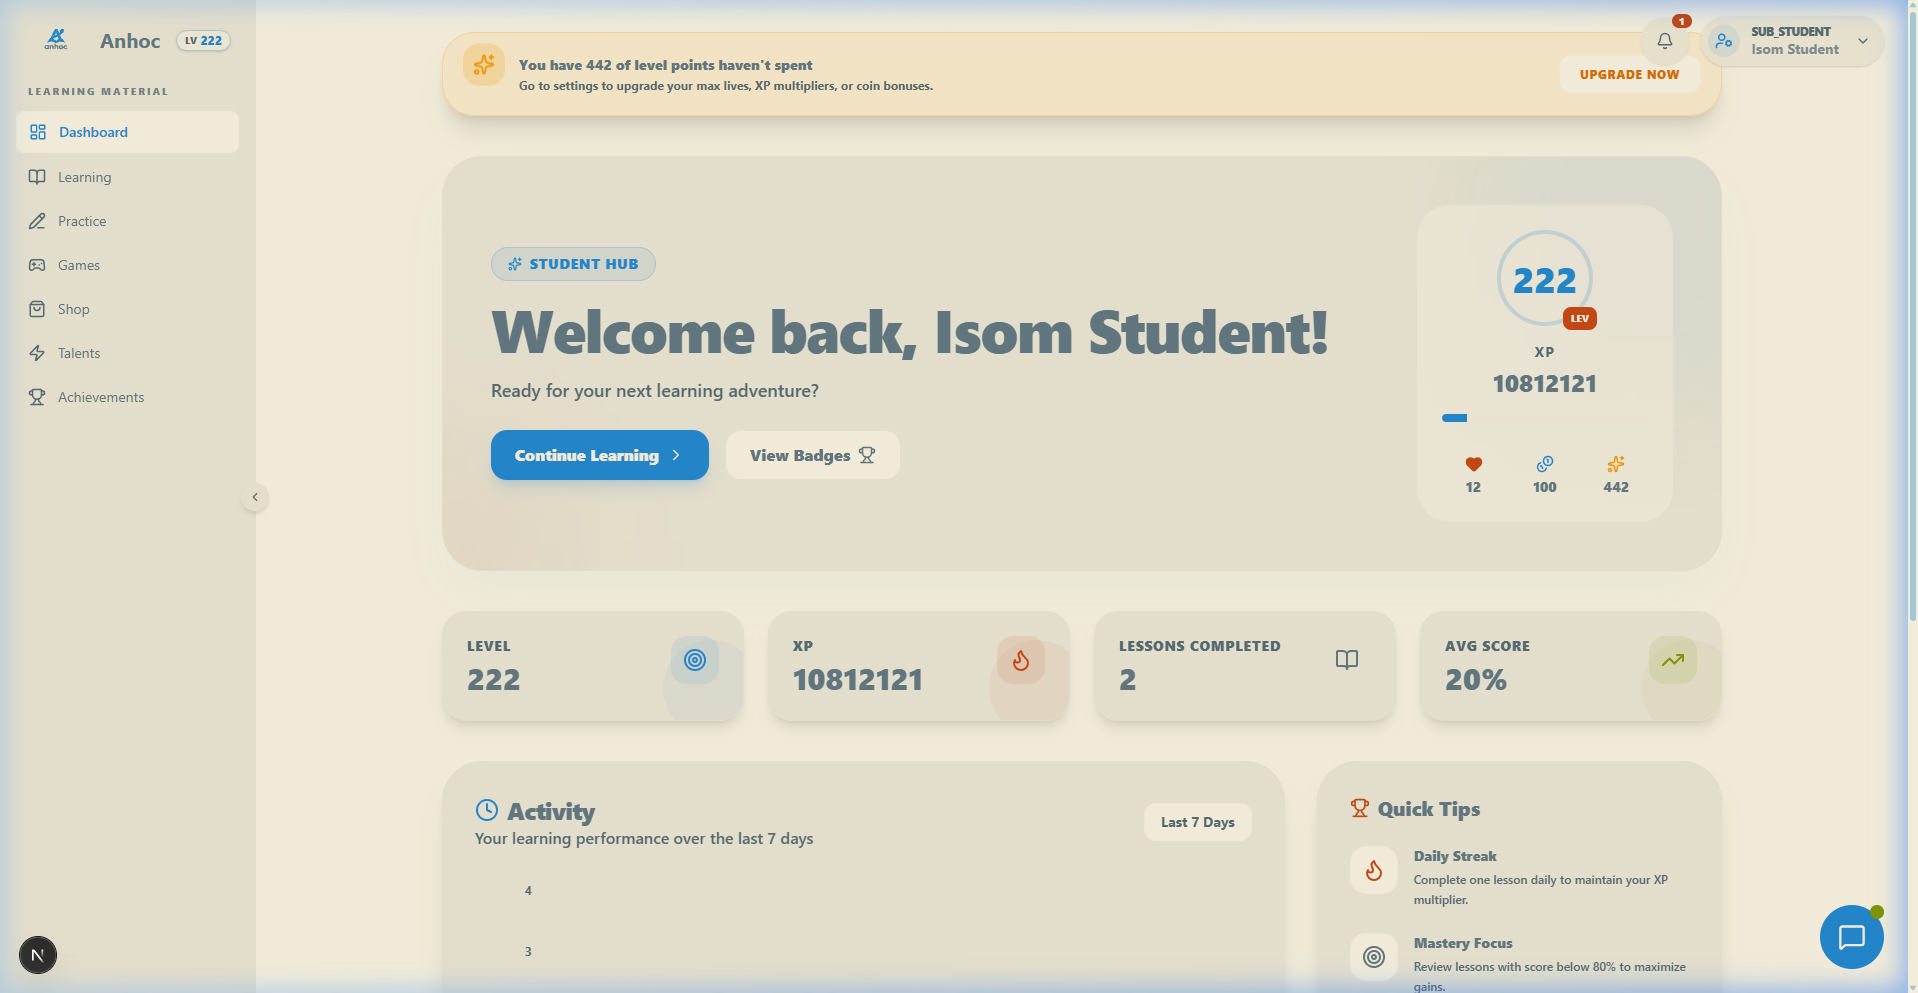
\includegraphics[width=\textwidth]{images/student_dashboard.png}
        \caption{Student dashboard showing XP, levels, and achievements.}
        \label{fig:student_dashboard}
    \end{minipage}
    \hfill
    \begin{minipage}{0.48\textwidth}
        \centering
        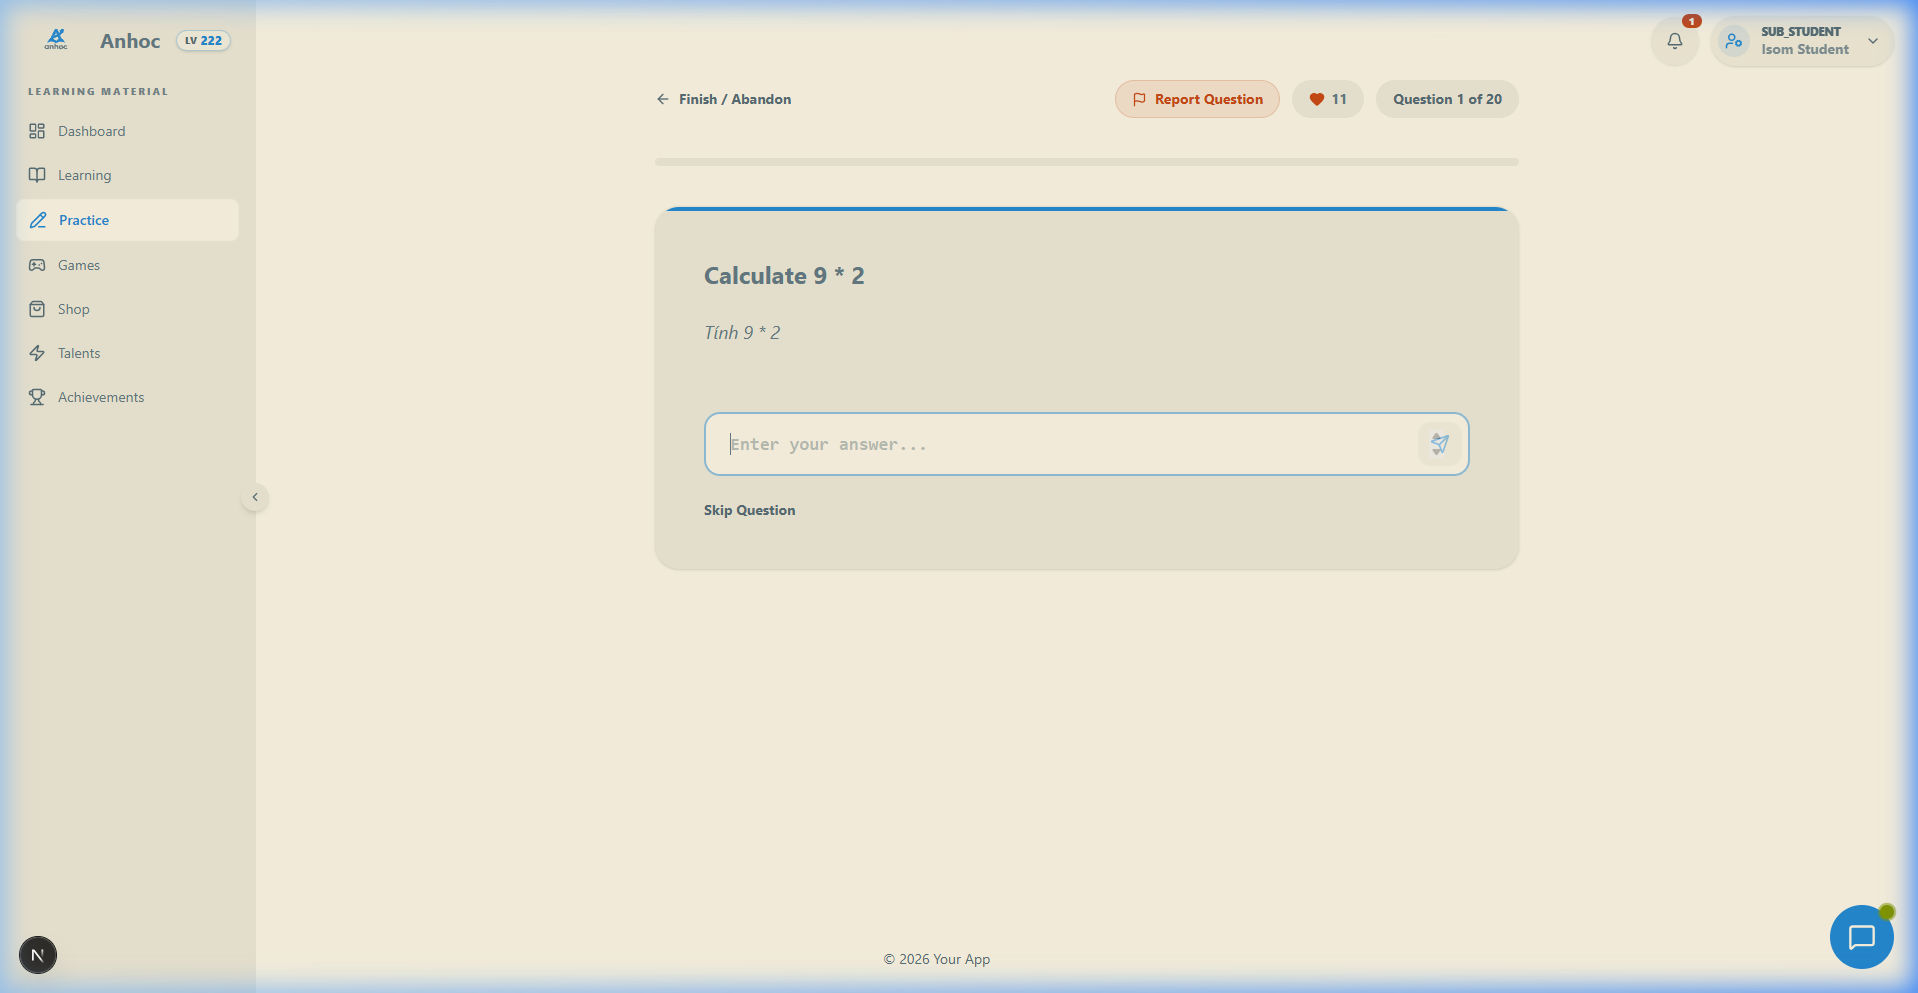
\includegraphics[width=\textwidth]{images/lesson_practice.png}
        \caption{Interactive mathematics practice interface.}
        \label{fig:lesson_practice}
    \end{minipage}
\end{figure}

\begin{figure}[H]
    \centering
    \begin{minipage}{0.48\textwidth}
        \centering
        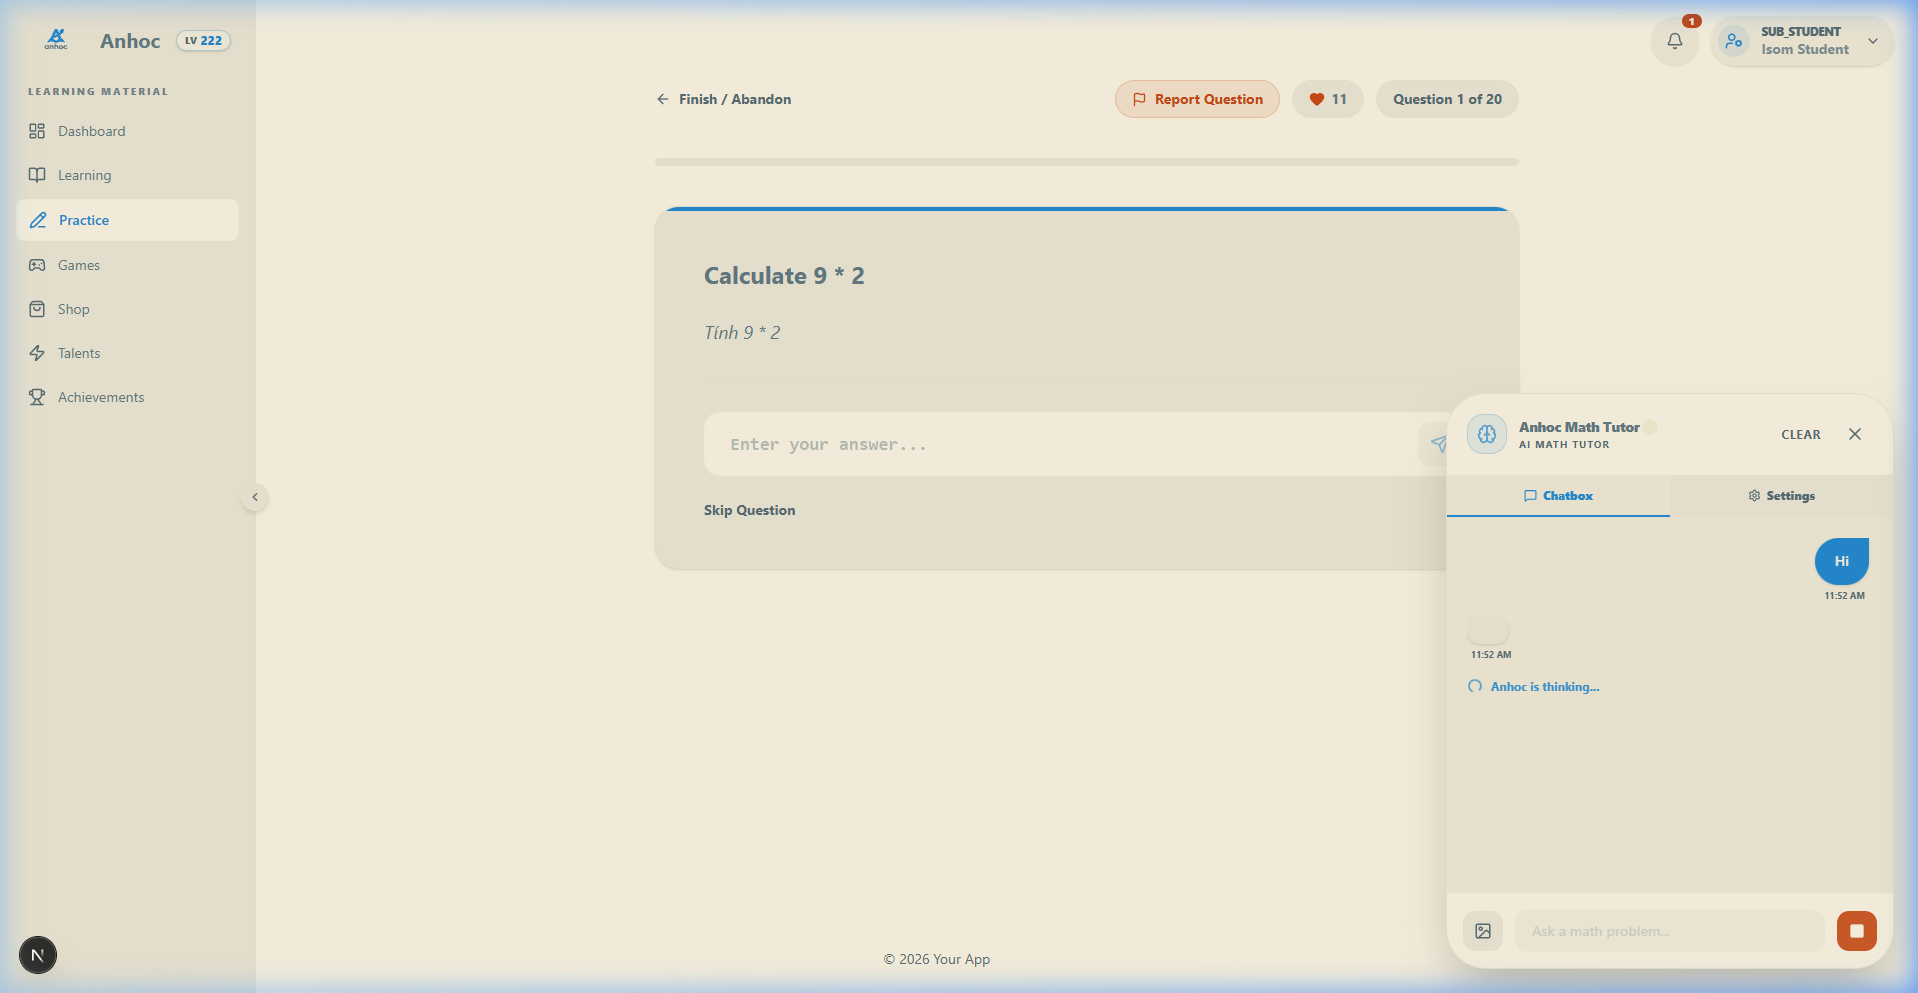
\includegraphics[width=\textwidth]{images/chatbot_widget.png}
        \caption{AI tutoring chatbot widget with reasoning.}
        \label{fig:chatbot_widget}
    \end{minipage}
    \hfill
    \begin{minipage}{0.48\textwidth}
        \centering
        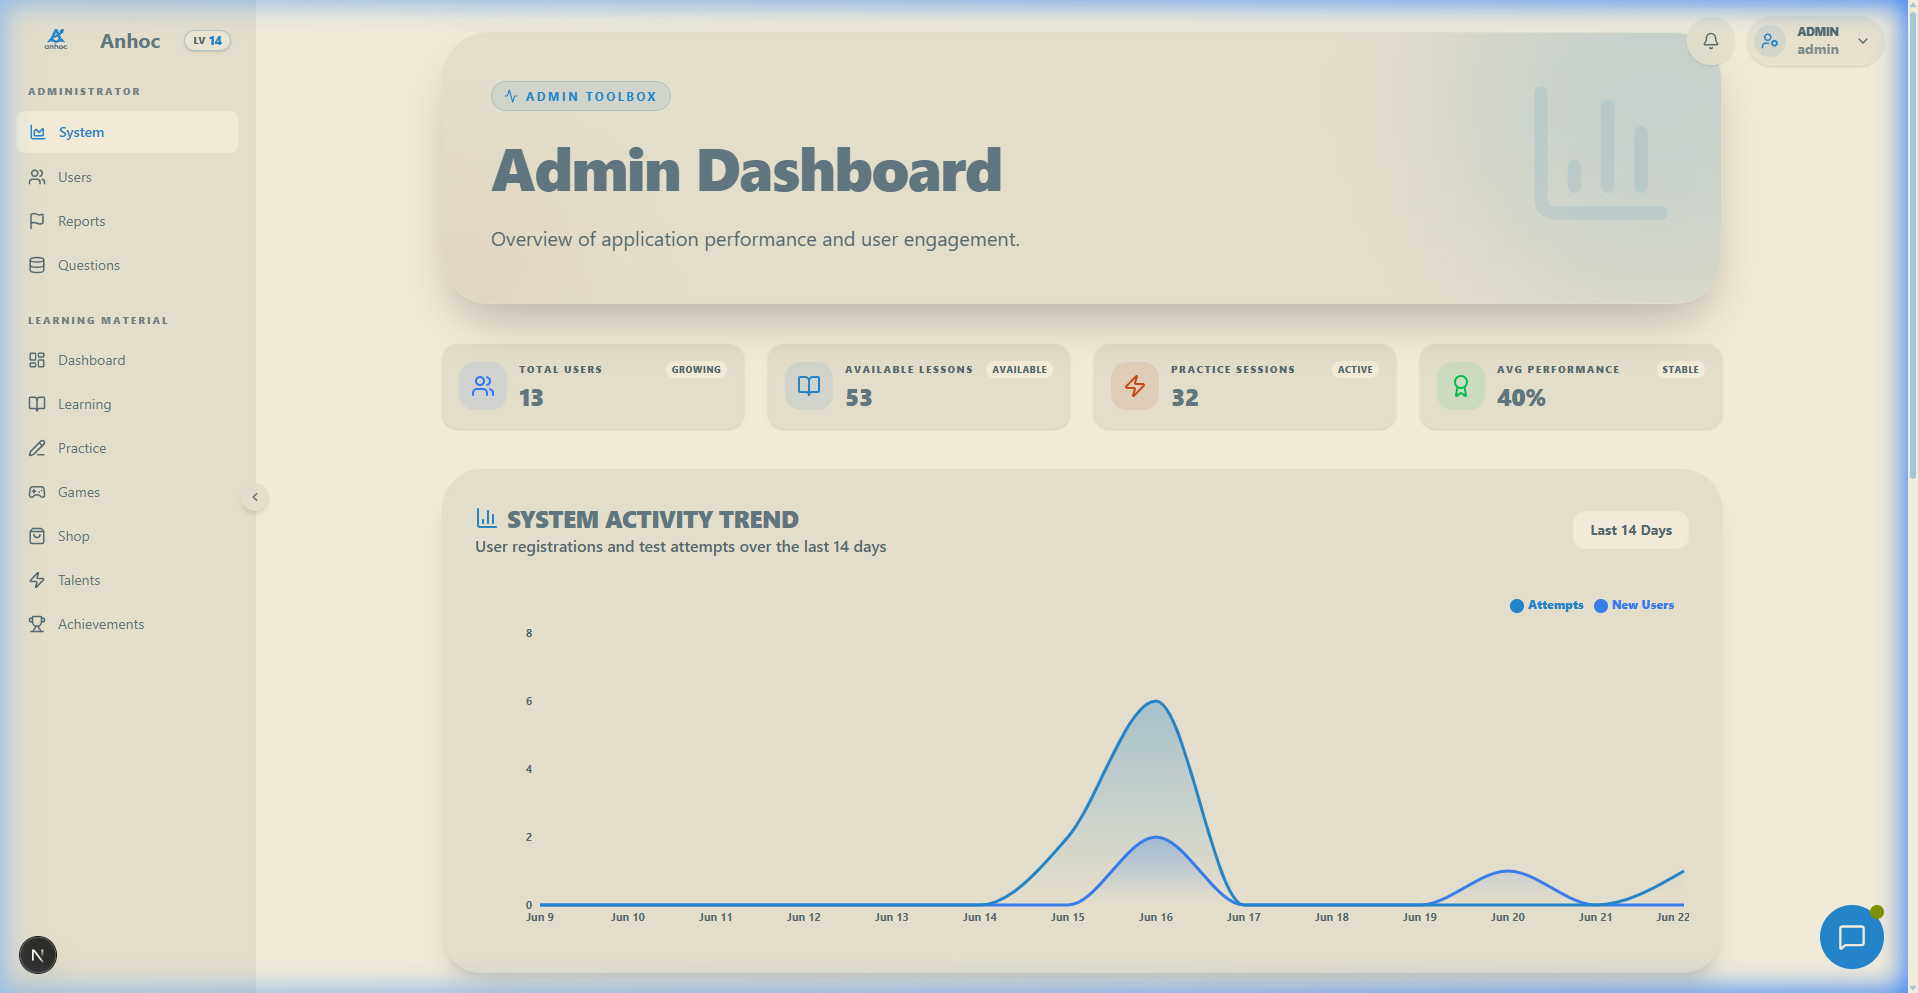
\includegraphics[width=\textwidth]{images/admin_dashboard.png}
        \caption{Administrative overview panel.}
        \label{fig:admin_dashboard}
    \end{minipage}
\end{figure}



\begin{thebibliography}{99}
\bibitem{anhoc-readme}
Anhoc project repository overview, \code{README.md}.

\bibitem{frontend-package}
Anhoc frontend package manifest and framework dependencies, \code{frontend/package.json}.

\bibitem{backend-package}
Anhoc backend package manifest and runtime dependencies, \code{backend/package.json}.

\bibitem{nextjs-docs}
Vercel. \textit{Next.js Documentation: App Router}. Available at:
\url{https://nextjs.org/docs/app}. Accessed June 15, 2026.

\bibitem{react-docs}
Meta Platforms, Inc. and contributors. \textit{React Documentation}. Available at:
\url{https://react.dev/learn}. Accessed June 15, 2026.

\bibitem{express-docs}
OpenJS Foundation and Express contributors. \textit{Express.js 5.x API Reference}. Available at:
\url{https://expressjs.com/en/api/}. Accessed June 15, 2026.

\bibitem{prisma-docs}
Prisma. \textit{Prisma ORM Documentation}. Available at:
\url{https://www.prisma.io/docs/orm}. Accessed June 15, 2026.

\bibitem{postgresql-docs}
PostgreSQL Global Development Group. \textit{PostgreSQL 18 Documentation}. Available at:
\url{https://www.postgresql.org/docs/current/index.html}. Accessed June 15, 2026.

\bibitem{jwt-rfc}
M. Jones, J. Bradley, and N. Sakimura. \textit{RFC 7519: JSON Web Token (JWT)}.
RFC Editor, May 2015. Available at: \url{https://www.rfc-editor.org/info/rfc7519/}.

\bibitem{jwt-bcp}
N. Sheffer, D. Hardt, and M. Jones. \textit{RFC 8725: JSON Web Token Best Current Practices}.
RFC Editor, February 2020. Available at: \url{https://www.rfc-editor.org/info/rfc8725/}.

\bibitem{mathjs-docs}
\textit{mathjs Documentation}. Available at: \url{https://mathjs.org/docs/}. Accessed June 15, 2026.

\bibitem{nextintl-docs}
Jan Amann and contributors. \textit{next-intl Documentation: Getting Started}. Available at:
\url{https://next-intl.dev/docs/getting-started}. Accessed June 15, 2026.

\bibitem{backend-server}
Anhoc backend bootstrap implementation, \code{backend/server.ts}.

\bibitem{backend-schema}
Anhoc database schema and Prisma models, \code{backend/prisma/schema.prisma}.

\bibitem{backend-auth}
Anhoc authentication and authorization middleware, \code{backend/middleware/auth.ts}.

\bibitem{backend-math}
Anhoc math generation and answer evaluation service, \code{backend/services/mathService.ts}.

\bibitem{chatbot-spec}
Anhoc tutoring chatbot specification and implementation, \code{chatbot/SPEC.md},
\code{chatbot/README.md}, and \code{chatbot/main.py}.

\bibitem{chatbot-widget}
Anhoc tutoring widget integration in the frontend, \code{frontend/src/components/feature/ChatbotWidget.tsx}.

\bibitem{technical-design}
Anhoc technical design document, \code{docs/TDD/technical-design.md}.
\end{thebibliography}

\end{document}
